  \let\negmedspace\undefined
\let\negthickspace\undefined
\documentclass[journal]{IEEEtran}
\usepackage[a5paper, margin=10mm, onecolumn]{geometry}
\usepackage{lmodern} % Ensure lmodern is loaded for pdflatex
\usepackage{tfrupee} % Include tfrupee package

\setlength{\headheight}{1cm} % Set the height of the header box
\setlength{\headsep}{0mm}     % Set the distance between the header box and the top of the text

\usepackage{gvv-book}
\usepackage{gvv}
\usepackage{cite}
\usepackage{amsmath,amssymb,amsfonts,amsthm}
\usepackage{algorithmic}
\usepackage{graphicx}
\usepackage{textcomp}
\usepackage{xcolor}
\usepackage{txfonts}
\usepackage{listings}
\usepackage{enumitem}
\usepackage{mathtools}
\usepackage{gensymb}
\usepackage{comment}
\usepackage[breaklinks=true]{hyperref}
\usepackage{tkz-euclide} 
\usepackage{listings}                                      
\def\inputGnumericTable{}                                 
\usepackage[latin1]{inputenc}                                
\usepackage{color}                                            
\usepackage{array}                                            
\usepackage{longtable}
\usepackage{multicol}
\usepackage{calc}                                             
\usepackage{multirow}                                         
\usepackage{hhline}                                           
\usepackage{ifthen}                                           
\usepackage{lscape}
\begin{document}
	
	\bibliographystyle{IEEEtran}
	\vspace{3cm}
	
	\title{11.16.3.3.4}
	\author{EE24BTECH11063 - Y. Harsha Vardhan Reddy }
	% \maketitle
	% \newpage
	% \bigskip
	{\let\newpage\relax\maketitle}
	
	\renewcommand{\thefigure}{\theenumi}
	\renewcommand{\thetable}{\theenumi}
	\setlength{\intextsep}{10pt} % Space between text and floats
	
	
	\numberwithin{equation}{enumi}
	\numberwithin{figure}{enumi}
	\renewcommand{\thetable}{\theenumi}
	
	
\textbf{Question}:\\
A die is rolled, Find the probability that a number greater than 6 will appear \\
\textbf{Solution: }\\
\textbf{Textual solution: }\\
Probability of a given event 'A'(A: Outcome is greater than 6),\\
\begin{align}
    \text{P(A)}=\frac{0}{6}=0
\end{align}
\textbf{Textual solution: }\\

\section*{Introduction}
The task involves simulating the roll of a single die using a C program, compiling it into a shared object (.so) file, and then using Python to call this function. The Python code processes the results and generates a probability distribution plot for outcomes \(1, 2, 3, 4, 5, 6\), and \textgreater6.

\section*{C Code Description}
The C program generates random outcomes for rolling a single die, where the possible outcomes range from \(1\) to \(10\). Outcomes are categorized as follows:\\
The program uses the \texttt{rand()} function to generate random numbers and increments the respective indices of the results array based on the generated outcome.

\section*{Python Code Description}
The Python code is responsible for:
\begin{enumerate}
    \item Loading the shared object file generated from the C program using the \texttt{ctypes} library.
    \item Calling the C function to roll the die for a specified number of trials (e.g., \(10,000\)).
    \item Retrieving the results from the C function as an array.
    \item Calculating the probabilities for each outcome using the formula:
    \[
    P(\text{outcome}) = \frac{\text{frequency of outcome}}{\text{total trials}}
    \]
    \item Plotting the probability distribution using \texttt{matplotlib}.
\end{enumerate}

\section*{Graphical Output}
The Python code generates a bar chart where:
\begin{itemize}
    \item The x-axis represents the outcomes: \(1, 2, 3, 4, 5, 6, \textgreater6\).
    \item The y-axis represents the probabilities of each outcome, ranging from \(0\) to \(1\).
    \item Each bar height corresponds to the probability of the respective outcome.
\end{itemize}

\section*{Key Points}
\begin{itemize}
    \item Using the C program ensures efficient computation of outcomes for large numbers of trials.
    \item The shared object file facilitates seamless integration with Python, leveraging Python's powerful visualization capabilities.
    \item The probabilities provide a normalized representation of the frequency distribution, making it easier to interpret the results.
\end{itemize}

\section*{Conclusion}
This task demonstrates the integration of C and Python for simulating and visualizing a probabilistic experiment. By combining the computational efficiency of C with the graphical capabilities of Python, we achieve an effective solution for analyzing and representing data. The code clearly shows that the probability of the given event is equal to \textbf{zero}

	\begin{figure}[h!]
		\centering
		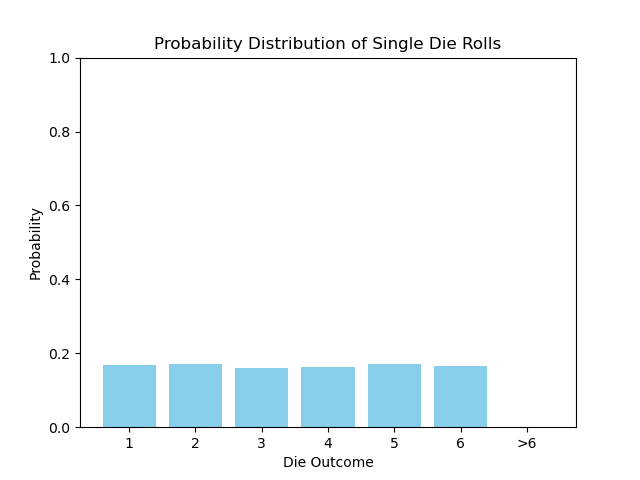
\includegraphics[width=\columnwidth]{figs/fig1.png}
		\caption{Solution of the system of linear equations}
		\label{stemplot}
	\end{figure}
	
\end{document}  
